\documentclass{template}
\usepackage{graphicx}

\project{Comthings}
\title{Hitag-2 cryptanalyse}
\author{Kaci Amaouche}
\faculty{Arithmétique, codage et cryptologie}
\department{Mathématiques}
\setlength{\hoffset}{-18pt}        
\setlength{\oddsidemargin}{0pt} % Marge gauche sur pages impaires
\setlength{\evensidemargin}{9pt} % Marge gauche sur pages paires
\setlength{\marginparwidth}{54pt} % Largeur de note dans la marge
\setlength{\textwidth}{481pt} % Largeur de la zone de texte (17cm)
\setlength{\voffset}{-18pt} % Bon pour DOS
\setlength{\marginparsep}{7pt} % Séparation de la marge
\setlength{\topmargin}{0pt} % Pas de marge en haut
\setlength{\headheight}{13pt} % Haut de page
\setlength{\headsep}{10pt} % Entre le haut de page et le texte
\setlength{\footskip}{27pt} % Bas de page + séparation
\setlength{\textheight}{708pt} % Hauteur de la zone de texte (25cm)
\begin{document}

\chapter{Définition et présentation du système Hitag-2}
\section{Description Hitag-2}
\subsubsection{Définition}
\baselineskip=16pt

Hitag-2 est un algorithme de chiffrement par flot utilisé dans les systèmes RKE (Remote Keyless Entry), également connus sous le nom de systèmes d'ouverture à distance des véhicules. Il a été conçu par Mikron, une société autrichienne qui a été acquise par Philips Semiconductors en 1995.

\subsubsection{Description de l'algorithme}
\baselineskip=16pt

L'algorithme Hitag-2 est le cousin de "Crypto1", qui est utilisé dans les cartes NFC Mifare Classic. Il repose sur une clé secrète de 48 bits, un état interne de 48 bits, une fonction linéaire basée sur un registre à décalage à rétroaction linéaire (LFSR) agissant sur cet état interne, et une fonction de filtrage non linéaire $f$. Cette fonction de filtrage prend 20 bits en entrée et génère 1 bit en sortie à chaque cycle d'horloge.

La fonction de sortie peut être visualisée comme une composition de deux niveaux de multiplexeurs différents. Les quatre bits d'entrée des fonctions $fa$ et $fb$ sont utilisés pour adresser et sélectionner l'un des bits de données stockés dans l'état interne. Ces fonctions permettent de sélectionner 5 bits. La fonction de sortie $fc$ prend ensuite les données provenant de $f$a et $fb$ (5 bits) en entrée et produit 1 bit de données en sortie.

L'algorithme est capable de générer autant de bits que nécessaire pour un chiffrement par flot grâce à son keystream. Cependant, seuls les 32 premiers bits du keystream $ks$ sont utilisés comme authentifiant dans le contexte d'utilisation de RKE (la figure ci-dessous décrit la structure de cet algorithme).


\begin{figure}
    \centering
    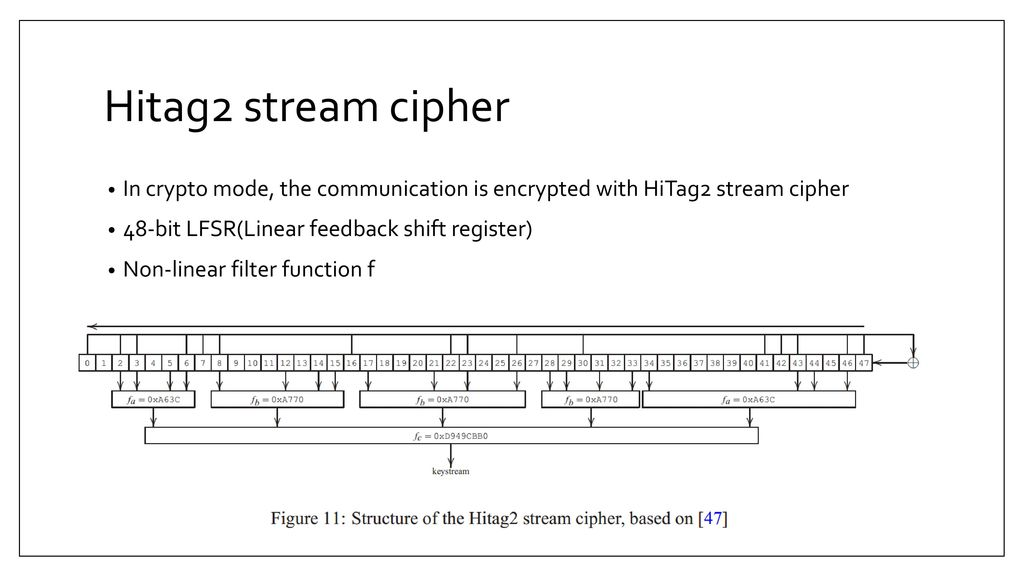
\includegraphics[width=\textwidth]{slide_15.jpg}
    \caption{Hitag-2 structure algorithmique}
    \label{fig:image}
\end{figure}

\subsubsection{Préliminaires}
\begin{itemize}
    \item Le corps fini à deux éléments 0 et 1 est noté \(F_2\). L'opération d'addition XOR dans ce corps est représentée par le symbole \(\oplus\). L'opération de multiplication (ET logique) est représentée par le symbole \(\&\). \(F_2^n\) représente l'ensemble résultant du produit cartésien de \(F_2\) pris \(n\) fois : \(F_2^n = \(F_2\) \times \ldots \times \(F_2\) (\(n\) fois). 
    \item Une chaîne \(x\) composée de \(n\) bits a son \(i\)-ème bit noté \(x_i\), avec \(0 \leq i < n\). La chaîne est représentée par \(x_0 \ldots x_{n-1}\). Par exemple, en notation hexadécimale, \(0x01\) (équivalente à \(00000001\)).
    \item Selon la notation précédente, \((0x010000)_i\) sélectionne le \(i\)-ème bit de la chaîne de 24 bits \(0x010000\). Ainsi, \((0x010000)_7\) est égal à 1, et \((0x010000)_i\) est égal à 0 pour tout \(i\) compris entre 0 et 23, à l'exception de \(i = 7\), car la chaîne de 24 bits \(0x010000\) est représentée par \((000000010000000000000000)\).
    \item L'opération d'addition \(\oplus\) entre deux chaînes de bits \(x\) et \(y\) de même taille \(n\) est définie comme l'addition bit à bit : chaque bit de \(x\) est combiné avec le bit correspondant de \(y\) pour donner une chaîne de \(n\) bits résultante.
    \item La concaténation de deux chaînes de bits \(x\) et \(y\), qui peuvent avoir des tailles différentes, est indiquée par \(xy\) ou \(x||y\).
\end{itemize}

\subsubsection{Fonctionnement}
\baselineskip=16pt

Tout d'abord, nous commençons par présenter formellement la définition de la fonction de rétroaction linéaire \(L\) et de la fonction non linéaire \(f\). Ensuite, nous procédons à une explication détaillée du fonctionnement de ce système.

\begin{itemize}
    \item La fonction \(L\) est définie de \(F_2^{48} \to F_2\) par \(L(x_0...x_{47}) = x_0 \oplus x_2 \oplus x_3 \oplus x_6 \oplus x_7 \oplus x_8 \oplus x_{16} \oplus x_{22} \oplus x_{23} \oplus x_{26} \oplus x_{30} \oplus x_{41} \oplus x_{42} \oplus x_{43} \oplus x_{46} \oplus x_{47}\).
    \item La fonction non linéaire \(f\) est définie de \(F_2^4 \to F_2\) par
    
    \(f(x) = fc(fa(x_{2}x_{3}x_{5}x_{6}), fb(x_{8}x_{12}x_{14}x_{15}), fb(x_{17}x_{21}x_{23}x_{26})
    ,fb(x_{28}x_{29}x_{31}x_{33}), fa(x_{34}x_{43}x_{44}x_{46}))\), où \(fa\), \(fb\), \(fc\) sont des sous-fonctions définies par :
    
    \begin{itemize}
        \item \(fa\) de \(F_2^4 \to F_2\) : \(fa(i)=(0xA63C)_i\)
        \item \(fb\) de \(F_2^4 \to F_2\) : \(fb(i)=(0xA770)_i\)
        \item \(fc\) de \(F_2^5 \to F_2\) : \(fc(i)=(0xD949CBB0)_i\)
    \end{itemize}
\end{itemize}
\baselineskip=16pt
Maintenant, nous allons expliquer le déroulement de ce système qui est basé sur les puces de type PCF7946/7947. L'algorithme prend trois paramètres en entrée : un vecteur d'initialisation \(iv\) de 32 bits, une clé \(k\) de 48 bits et un identifiant \(id\) de 32 bits.

Le fonctionnement se déroule en trois phases : la phase d'initialisation, la phase de randomisation et la phase nominale.

Lors de la première et de la deuxième phase, l'état interne du registre évolue pendant 80 cycles et seule la fonction \(f\) intervient.

La phase d'initialisation consiste à assigner les valeurs de l'identifiant \(id\) aux 32 premiers bits de l'état interne, puis les 16 premiers bits de la clé \(k\) aux bits restants du registre (31-47).

La phase de randomisation consiste à faire évoluer l'état du registre pendant 32 cycles d'horloge, et plus exactement les 32 derniers bits (on verra dans la suite que cela représente une faille dans le système car les 16 premiers bits de l'état interne ne varient pas durant cette phase et ces bits sont ceux de la clé \(k\)), en faisant un XOR entre les valeurs du vecteur d'initialisation \(iv\) avec les 32 derniers bits de la clé \(k\) et la sortie de la fonction non linéaire \(f\). Plus formellement (en notant "a" l'état du registre), on peut décrire cette variation mathématiquement par :

\[a_{48+i}=k_{16+i} \oplus iv_i \oplus f(a_i \ldots a_{i+47})\]

Dans la phase nominale, le déroulement consiste à effectuer des décalages avec le LFSR sur l'état interne du registre. Et dans le cas de RKE, on prend que les 32 premiers bits sortant de l'algorithme. Plus formellement, on peut écrire :

\[Ks(i)=f(a_{32+i} \ldots a_{79+i})\]

Le format de la trame du paquet radio envoyé par le PCF7946/7947 est donné dans la figure ci-dessous.

\begin{figure}
    \centering
    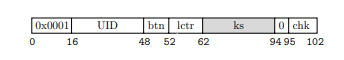
\includegraphics[width=\textwidth]{tempsnip.png}
    \caption{Trame PCF7946/7947}
    \label{fig:image}
\end{figure}

\subsubsection{Explications relatives au paquet envoyé par le PCF}
On voit que le paquet se compose de 6 champs, on donnera une définition de chacun.

\begin{itemize}
    \item Le premier (\(0x0001\)) qu'on note SYNC, est une séquence de synchronisation de 16 bits envoyée en préambule pour assurer la bonne synchronisation d'horloge du côté du récepteur.
    \item UID représente l'identifiant unique.
    \item btn représente l'identifiant du bouton codé sur 4 bits.
    \item lctr représente les 10 bits de points faibles du compteur RKE.
    \item ks est le keystream de 32 bits généré par l'algorithme.
    \item chk est le checksum codé sur 8 bits qui est le XOR de tous les paquets précédents hors SYNC.
\end{itemize}

La taille de la trame est de 102 bits et 102 n'étant pas un multiple de 8, on rajoute un padding '10' juste après ks afin que chk ait un sens.


\section{Faiblesses cryptographiques}
\baselineskip=16pt
Dans cette section, nous allons discuter des vulnérabilités et des faiblesses cryptographiques du système. En outre, nous aborderons également des notions connexes qui sont liées à ces faiblesses.

Le protocole HITAG 2 offre trois modes de fonctionnement : le mode public, le mode password et le mode crypto.

En mode public, le contenu des pages de données utilisateur est simplement diffusé par le transpondeur une fois qu'il est alimenté.

En mode password, le lecteur et le transpondeur s'authentifient mutuellement en échangeant leurs mots de passe. La communication est effectuée en clair, ce qui rend cette procédure d'authentification vulnérable aux attaques de rejeu.

En mode crypto, le lecteur et le transpondeur effectuent une authentification mutuelle à l'aide d'une clé partagée de 48 bits. La communication entre le lecteur et le transpondeur est chiffrée à l'aide d'un chiffre de flux propriétaire.

Nous nous concentrons sur le mode crypto. Notre objectif est d'analyser le système et de détecter toutes les faiblesses et vulnérabilités mathématiques qui pourraient exister dans ce mode.

Afin de mieux comprendre l'une de ces faiblesses, on doit comprendre le protocole d'authentification.

Dans ce protocole, le lecteur commence la communication en envoyant une commande d'authentification, à laquelle le transpondeur répond en envoyant son identifiant. À partir de ce point, la communication est chiffrée en utilisant le keystream par une opération de XOR. Le lecteur répond avec son défi chiffré (\(nR\)) et la réponse (\(aR = 0xFFFFFFFF\)), également chiffrée, pour prouver sa connaissance de la clé. Le transpondeur termine en envoyant sa réponse chiffrée (\(aT\)), correspondant au défi du lecteur.

\begin{figure}
    \centering
    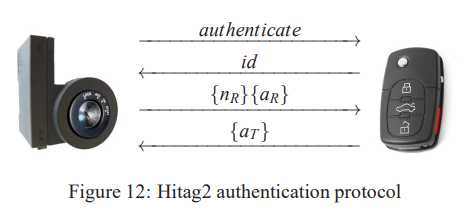
\includegraphics[width=\textwidth]{Capture.PNG}
    \caption{Hitag-2 protocole d'authentification}
    \label{fig:image}
\end{figure}

\subsubsection{Taille des clés}

\begin{itemize}
    \item L'état interne de 48 bits : l'état interne du chiffrement ne fait que 48 bits, ce qui le rend vulnérable à certaines attaques.
\end{itemize}

\subsubsection{Dépendance entre les sessions}

\begin{enumerate}
    \item Les bits LFSR (Linear Feedback Shift Register) du chiffrement ne sont pas complètement initialisés à chaque nouvelle session, ce qui crée une dépendance entre les différentes sessions.
    \item Les bits LFSR de 0 à 15 restent constants à travers différentes sessions, et seuls les bits LFSR de 16 à 47 varient, ce qui crée une forte dépendance entre eux.
\end{enumerate}

\subsubsection{Faible degré d'utilisation des bits de l'état interne dans la fonction de filtrage \(f\)}

\begin{enumerate}
    \item Faibles variations de \(ks\) lors de faibles variations des entrées \(id\) et \(iv\).
    \item À l'issue de la phase d'initialisation, l'état du registre interne est constant pour toutes les sessions d'un même transpondeur.
\end{enumerate}

\section{Attaques possibles}

Le système Hitag-2 présente plusieurs vulnérabilités majeures et est sujet à différentes attaques.

\subsection{Attaque par recherche exhaustive}
\baselineskip=16pt
La faible taille de la clé de 48 bits rend le système vulnérable à une attaque par recherche exhaustive. Cette attaque consiste à utiliser seulement 2 triplets (id, iv, ks) pour récupérer la clé k complète. Cependant, un seul triplet ne suffit pas pour retrouver de manière non ambiguë la clé k en raison des collisions possibles. Ainsi, un deuxième triplet est nécessaire pour lever cette ambiguïté. Des recherches exhaustives ont été réalisées sur différents types de processeurs, prenant plusieurs mois sur un processeur standard, mais seulement quelques heures sur une carte graphique performante.

\subsection{Attaques algébriques}
\baselineskip=16pt
Le système Hitag-2 est également vulnérable aux attaques algébriques. Ces attaques exploitent les équations booléennes quadratiques multivariées qui décrivent les liens entre la sortie ks et les entrées id, iv et k. Des recherches récentes ont montré que ces équations peuvent être simplifiées dans le cas de Hitag-2, facilitant ainsi le travail d'un solveur SAT. Le temps estimé pour résoudre ces équations est d'environ 6 heures en utilisant 16 paquets avec iv choisi, ou 45 heures avec 4 paquets aléatoires. Des attaques algébriques étendues ont également été proposées en utilisant des solveurs spécifiques aux algorithmes cryptographiques. Toutefois, peu de détails sont disponibles sur le contexte précis de ces attaques.

\subsection{Attaques marginales}

Les attaques plus marginales, telles que les attaques par Time Memory Trade Offs et les cube attacks, ne sont pas détaillées dans cet article. Les attaques par Time Memory Trade Offs nécessitent un contexte spécifique où un oracle de keystream fournit une sortie de grande taille, tandis que les cube attacks nécessitent 500 traces générées à partir d'iv choisis.

\subsection{Attaques par corrélation}
\baselineskip=16pt
L'idée principale de la cryptanalyse par corrélation est de réduire considérablement l'espace de recherche en identifiant des clés candidates ayant un bon score de corrélation. Ce score est calculé en comparant les bits de sortie observés ks avec les bits de clé devinés. Le processus de filtrage permet de sélectionner les candidats les plus plausibles et d'éliminer les moins plausibles lors du passage d'une génération de bits à une autre.

Le calcul du score est réalisé pour des clés candidates de taille variable, de 16 à 48 bits. Par exemple, pour les clés candidates de 16 bits, les bits devinés agissent sur les bits de keystream ks correspondants, et le score est calculé en moyennant les sorties possibles de la fonction de filtrage f. Ce calcul est étendu aux autres clés candidates de taille supérieure, en ne conservant que les meilleurs candidats à chaque étape.

L'attaquant utilise un tableau de taille fixe pour stocker les candidats et élimine progressivement ceux ayant le score le plus faible. Cette contrainte permet de restreindre l'espace de recherche. À la dernière génération, il ne reste que très peu de candidats avec un score élevé, et la bonne clé peut être identifiée par une vérification exhaustive.

Il est important de noter que la connaissance complète de l'IV n'est pas requise pour cette cryptanalyse, car la partie haute du compteur CNTRH n'est pas transmise par le transpondeur. Cependant, les auteurs ont proposé une approche pour estimer la valeur de CNTRH en fonction de l'âge du véhicule, ce qui permet de contourner ce problème. Ainsi, l'attaquant peut relancer la cryptanalyse en utilisant des IV forgés selon des hypothèses plausibles de CNTRH pour trouver la bonne clé.

Le temps de cryptanalyse reste de l'ordre de quelques dizaines de minutes si le nombre d'hypothèses est faible, ce qui a été observé dans les tests sur les véhicules étudiés par les auteurs.


\chapter{Attaque pratique sur Hitag-2}
\section{L'attaque guess and determine dans le cas général}
\baselineskip=16pt
Dans cette partie, nous nous concentrons sur l'attaque Guess and Determine, une méthode redoutable utilisée par les cybercriminels pour infiltrer les systèmes sécurisés. Nous décrivons en détail les mécanismes sous-jacents de cette attaque sophistiquée afin d'offrir une compréhension approfondie de son fonctionnement et de ses implications sur la sécurité informatique.


À travers une analyse rigoureuse, nous examinons les différentes phases de l'attaque Guess and Determine, en mettant notamment l'accent sur la phase de "devinette" où l'attaquant tente de trouver les valeurs appropriées pour exploiter les vulnérabilités du système. Nous mettons en évidence les techniques et les outils couramment utilisés par les attaquants pour réduire le nombre de possibilités, augmentant ainsi leurs chances de réussite.


De plus, nous explorons les conséquences potentielles de l'attaque Guess and Determine sur les systèmes et les données sensibles. Nous examinons les scénarios réels où cette technique a été utilisée avec succès pour contourner les mesures de sécurité et compromettre des informations confidentielles.


Dans notre étude, nous présentons également un exemple pratique d'utilisation d'un chiffrement par flux (stream cipher) avec une clé de 16 bits. Nous démontrons comment il est possible de réduire la complexité totale de l'attaque, initialement de $2^{16}$, à seulement $2^{13}$. Ce cas concret illustre l'impact significatif de certaines techniques sur la sécurité des systèmes utilisant des clés de chiffrement relativement courtes.
\subsubsection{Exemple d'un chiffrement par flot}
\baselineskip=16pt
\begin{figure}
    \centering
    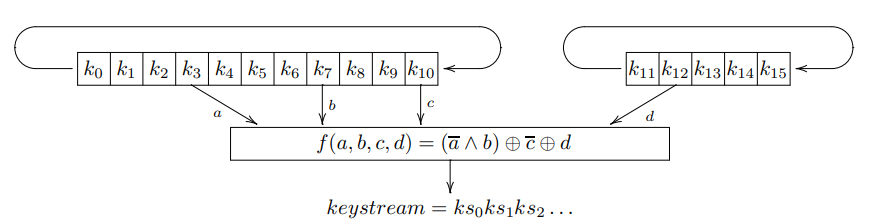
\includegraphics[width=\textwidth]{stream-cipher.PNG}
    \caption{Stream cipher}
    \label{fig:image}
\end{figure}

La présente illustration met en évidence le fonctionnement d'un système de chiffrement à flot utilisant une clé de 16 bits. Le système utilise une fonction non linéaire $f$ avec 4 bits en entrée, générant un bit à chaque cycle d'horloge.

À chaque cycle d'horloge, la fonction $f$ utilise les valeurs $a$, $b$, $c$ et $d$ en entrée. Dans chaque bloc (à gauche de 11 bits et à droite de 5 bits), les bits subissent un décalage vers la gauche sans que ces valeurs ne soient modifiées. Par exemple, à l'instant $t=1$, nous aurons un bloc de $k_1k_2k_3k_4k_5k_6k_7k_8k_9k_{10}k_0k_{12}k_{13}k_{14}k_{15}k_{11}$.

Lorsqu'un registre n'utilise pas son état interne complet pour calculer un keystream, cela le rend vulnérable à l'attaque Guess and Determine (G&D) (on verra pourquoi dans la suite).  

Dans le cadre de cette attaque, l'attaquant tente de deviner les bits utilisés ($a$, $b$, $c$, $d$), puis calcule la sortie et l'évalue par rapport au bit correspondant du flux de clés qui a été récupéré.

À chaque évaluation, un certain nombre de candidats sera éliminé, et seuls les bits supplémentaires nécessaires seront devinés. Cela permet de réduire le nombre de possibilités et de concentrer les efforts sur les bits restants.

\subsubsection{Explication de l'attaque}
\baselineskip=16pt
La fonction $f$ utilisée dans ce système, et dans la plupart des cas, est une fonction booléenne équilibrée. Cela signifie qu'elle renvoie autant de 0 que de 1. Ces fonctions sont choisies pour générer des nombres pseudo-aléatoires et pour être résistantes aux attaques statistiques.

Grâce à une attaque de force brute, la complexité serait de $2^{16}$, cependant, avec l'attaque Guess and Determine (G&D), nous pouvons la réduire à $2^{13}$ dans cet exemple donné.

Comme illustré dans la figure, la fonction $f$ nécessite 4 bits en entrée pour générer un bit $ks$ en sortie. Effectivement, étant donné que seulement 4 bits sont utilisés à chaque itération, il serait inutile d'essayer de deviner tous les bits en une seule fois. La force de l'attaque Guess and Determine repose précisément sur cette observation. L'attaquant se concentre sur la devinette des seuls bits utilisés à chaque itération et s'assure qu'ils produisent le même keystream. Cela permet de réduire considérablement la complexité de l'attaque, car seule une partie des bits est nécessaire pour obtenir le résultat désiré.

\subsubsection{Déroulement de l'attaque}
\baselineskip=16pt
Supposons qu'un attaquant dispose de la suite chiffrante $ks_0ks_1...ks_{15}$. Nous aurons uniquement besoin des 5 premiers $ks_0...ks_4$. Nous pouvons les écrire comme :

\begin{align*}
ks_0 &= f(k_3, k_7, k_{10}, k_{12}) \\
ks_1 &= f(k_4, k_8, k_0, k_{13}) \\
ks_2 &= f(k_5, k_9, k_1, k_{14}) \\
ks_3 &= f(k_6, k_{10}, k_2, k_{15}) \\
ks_4 &= f(k_7, k_0, k_3, k_{11})
\end{align*}

Nous observons que $ks_0$ est déterminé par les bits $k_3$, $k_7$, $k_{10}$ et $k_{12}$. L'attaquant doit donc deviner 16 candidats possibles ($2^4 = 16$). Supposons que $ks_0$ soit égal à 1. Dans ce cas, la moitié des 16 candidats sera éliminée grâce à l'équilibrage de la fonction $f()$. Ainsi, l'attaquant réussit à réduire le nombre de candidats potentiels à deviner à 8 ($2^3 = 8$).

De même pour $ks_1$, l'attaquant doit deviner les 4 bits $k_4$, $k_8$, $k_0$ et $k_{13}$. On constate que ces 4 bits sont complètement différents de ceux qui ont produit $ks_0$. Par conséquent, l'attaquant devra deviner parmi les 16 candidats possibles. Cependant, grâce à l'équilibrage de la fonction $f()$, la moitié des candidats peut être éliminée, ce qui réduit le nombre de candidats restants à $2^3 = 8$. L'attaquant a donc maintenant deviné une clé de 8 bits : $k_0$, $k_3$, $k_4$, $k_7$, $k_8$, $k_{10}$, $k_{12}$, $k_{13}$.

Contrairement aux 256 candidats possibles lorsque 8 bits sont inconnus, après avoir calculé les $2^7 = 128$ candidats possibles, on peut encore éliminer la moitié d'entre eux. Cela réduit le nombre de candidats restants à $2^6 = 64$.

L'adversaire applique la même technique pour le 3e bit $ks_2$. Il va deviner à nouveau une clé de 12 bits après $2^6 \times 2^4 = 2^{10}$ calculs, et la moitié sera éliminée, il en reste donc $2^9$ candidats pour une clé de 12 bits.

Pour le 4e bit $ks_3 = f(k_6, k_{10}, k_2, k_{15})$, l'adversaire n'aura que 3 bits à deviner car le $k_{10}$ a déjà été deviné précédemment pour calculer $ks_0$, ce qui fait $2^9 \times 2^3 = 2^{12}$, et après avoir évalué $ks_3$, l'espace des candidats diminue à $2^{11}$.

Il reste maintenant à déterminer $k_{11}$ (qui n'a pas encore été utilisé pour le calcul d'un $ks$). Sachant que $ks_4 = f(k_7, k_0, k_3, k_{11})$, l'adversaire n'aura qu'un bit à deviner, donc l'espace des candidats sera de $2 \times 2^{11} = 2^{12}$, puis il sera réduit à nouveau à $2^{11}$.

Finalement, nous avons une complexité totale de $2^4 + 2^7 + 2^{10} + (2 \times 2^{12}) = 2^{13}$.

\section{Guess and determine appliquée à Hitag-2}
\subsubsection{L'idée, le principe et le fonctionnement de l'attaque}
\baselineskip=16pt
L'idée de l'attaque repose sur l'inversion de la fonction booléenne non linéaire $f$ qui a 5 bits en entrée, et ces 5 bits sont les sorties des fonctions qui ont à leur tour 4 bits en entrée. Le but de l'attaque n'est pas de retrouver directement la clé secrète $K$, mais de retrouver l'état interne du registre, ce qui permet de trouver une clé équivalente.

Une fois que l'état interne réel est connu, cette idée peut être généralisée en inversant l'initialisation complète tout en devinant tous les bits de nonce inconnus. Cela permet d'obtenir une clé équivalente qui restera valide jusqu'à ce que tous les bits de compteur que nous pouvons observer débordent dans les bits d'état interne que nous avons devinés jusqu'à présent. Une telle clé équivalente, pour n'importe quelle valeur de $CNTR_L$, permet à l'adversaire de falsifier en moyenne les $2^9 = 512$ prochaines valeurs de $ks$. Après ce point, il existe plusieurs candidats pour une clé équivalente, car des inversions de bits en cascade dans les bits non observés du compteur peuvent s'être produites en incrémentant le compteur jusqu'au point de débordement des 10 bits les plus bas. À partir de tout nouveau triplet observé de $KS$, $BTN$ et $CNTR_L$, ainsi que des informations que nous avons utilisées pour calculer une clé équivalente précédente, une nouvelle clé équivalente peut être calculée de manière plus efficace.

Supposons que l'attaquant a intercepté une suite $ks_0ks_1...ks_{31}$. Il va donc essayer de deviner les bits qui produisent chaque bit $ks_i$. Il n'aura besoin que des 9 premiers bits $ks_0, ks_1...ks_8$. Plus formellement, selon le schéma du système Hitag-2, on peut écrire :

\begin{align*}
ks_0 &= f(a_2, a_3, a_5, a_6, a_8, a_{12}, a_{14}, a_{15}, a_{17}, a_{21}, a_{23}, a_{26}, a_{28}, a_{29}, a_{31}, a_{33}, a_{34}, a_{43}, a_{44}, a_{46}) \\
\end{align*}

Ces 20 bits sont l'entrée des sous-fonctions $fb$ et $fa$. On peut représenter ces bits sous forme de masques. Par exemple, si nous devons deviner $(a_0, a_1, a_5)$, nous utilisons le masque $(110001)$, où un bit à deviner est noté par 1.

Pour $ks_0$, il y aura donc $2^{20}$ candidats capables de produire ce bit. Cependant, la moitié des candidats sera éliminée lors de cette phase grâce au fait que $f$ est une fonction équilibrée.

Ensuite, pour $ks_1$, le registre est décalé à gauche et on peut écrire :

\begin{align*}
ks_1 &= f (a_3, a_4, a_6, a_7, a_9, a_{13}, a_{15}, a_{16}, a_{18}, a_{22}, a_{24}, a_{27}, a_{29}, a_{30}, a_{32}, a_{34}, a_{35}, a_{44}, a_{45}, a_{47}) \\
\end{align*}

Or, $a_3, a_6, a_{15}, a_{29}, a_{34}, a_{44}$ ont déjà été devinés, il y a donc 14 bits à deviner au lieu de 20.

À ce stade, l'attaquant aurait $2^{19} \times 2^{14} = 2^{33}$ candidats, puis il élimine la moitié des candidats, ce qui fait $2^{32}$ candidats restants.

En suivant la même logique, pour $ks_2$, il n'aura que 4 bits à deviner, ce qui fera $(2^{32} \times 2^4)/2 = 2^{35}$ candidats.

Pour $ks_3$, il n'aura que 3 bits à deviner, ce qui fera $(2^{35} \times 2^3)/2 = 2^{37}$ candidats.

À partir de $ks_3$ jusqu'à $ks_8$, il n'y a qu'un seul bit à deviner dans chaque étape (layer). Cet algorithme produira approximativement $2^{39}$ états possibles du LFSR qui ont généré la suite $ks_0...ks_8$. Il suffit donc de tester ces $2^{39}$ états contre les 23 bits restants $ks_9...ks_{31}$, ce qui produira une liste de $2^{16}$ états candidats.

Les deux figures suivantes présentent cette démarche. La première figure montre les bits à deviner dans chaque étape et ceux qui ont déjà été devinés, et la deuxième figure montre comment les décrire sous forme de masques.

\begin{figure}
    \centering
    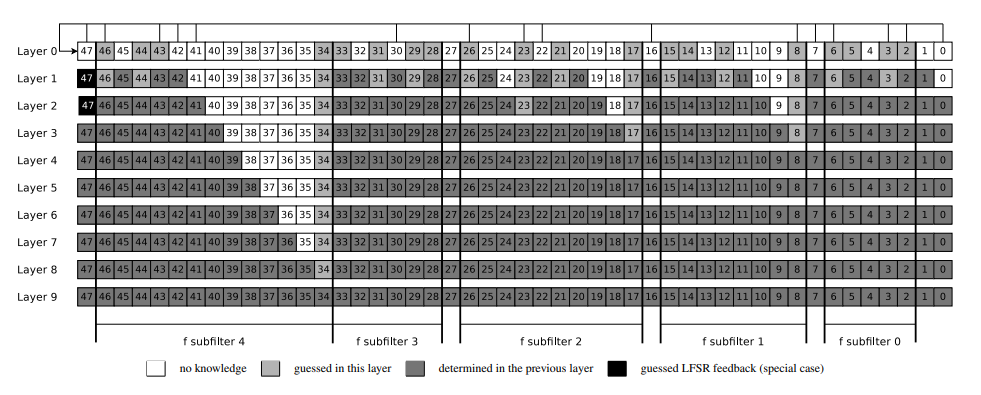
\includegraphics[width=\textwidth]{Layers.png}
    \caption{Layers}
    \label{fig:image}
\end{figure}

\begin{figure}
    \centering
    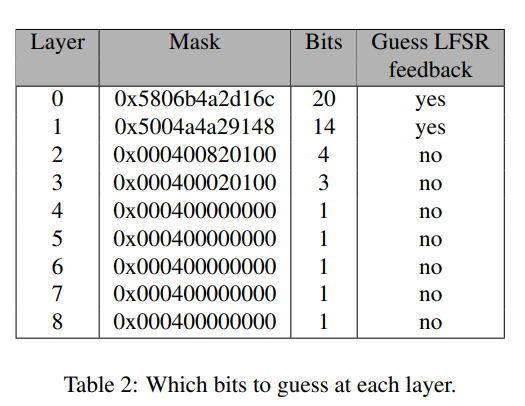
\includegraphics[scale=0.7]{mask.png}
    \caption{Bits à deviner}
    \label{fig:image}
\end{figure}

On peut ensuite réduire ces $2^{16}$ candidats à un seul candidat en suivant les étapes suivantes :

\begin{enumerate}
    \item \textbf{Recoupement des bits de nonce :} Le protocole utilisé dans le chiffrement Hitag2 utilise des bits de nonce qui se chevauchent. Cela signifie que certains bits du nonce sont utilisés à la fois pour le premier échantillon de flux de clés et pour le second échantillon de flux de clés. Ces informations de chevauchement permettent de réduire la liste des états de chiffrement potentiels à un seul état réel qui l'a généré.
    
    \item \textbf{Recul de chiffrement :} En utilisant un deuxième échantillon de flux de clés observé à partir du même émetteur et les informations de nonce observables utilisées pour générer les deux échantillons, le chiffrement peut être remonté en arrière en initialisant les bits de nonce connus les plus bas vers un état de chiffrement antérieur. À partir de cet état pré-initialisé, les bits de nonce observés associés au deuxième échantillon peuvent être chiffrés pour compléter un deuxième état initialisé. Si cet état génère le deuxième échantillon de flux de clés, les états initiaux corrects liés à ces deux échantillons sont identifiés.
    
    \item \textbf{Prédiction de l'état suivant :} Comme les bits de compteur les moins significatifs se trouvent dans les bits de nonce connus, il est possible d'incrémenter simplement ces bits de compteur et de choisir les bits de code de bouton appropriés pour prédire l'état de chiffrement initial suivant.
\end{enumerate}
\chapter{Implémentation}
Dans cette partie, on explique brièvement le principe de chaque attaque et optimisation possbile.
Une explication encore mieux détaillée est donnée dans les prorgrammes implémentés (.py, .c et .ipynb )
\section{Brute Force}
\baselineskip=16pt
Une clé de 48 bits est largement en dessous des standards modernes (et même de ceux des années 2000). Elle rend la recherche exhaustive accessible en un temps raisonnable. Celle-ci nécessite 2 triplets (id, iv, ks) pour récupérer les 48 bits de la clé K. Notons qu'un seul triplet ne suffit pas pour retrouver de manière non ambiguë K : puisque ks fait 32 bits, il y a en moyenne $2^{48-32} = 2^{16}$ clés K produisant le même triplet (id, iv, ks) à cause des collisions possibles, le second triplet permet donc de lever cette ambiguïté.

Cette attaque vise directement la clé secrète K. Elle itère de façon itérative sur toutes les $2^{48}$ clés possibles, et elle teste chacune d'entre elles pour voir si elle produit le bon keystream.
\section{GD version naive récursive}
\baselineskip=16pt


Voici une explication un peu plus formelle de cette implémentation :

\begin{enumerate}
  \item Tant que l'état n'est pas entièrement déterminé :
    \begin{enumerate}
      \item Déterminer tous les bits d'entrée du filtre de la couche en itérant un compteur.
      \item Étendre la valeur du compteur avec le masque de la couche en utilisant la fonction d'expansion.
      \item Combiner la valeur étendue avec l'état de la couche précédente.
      \item Calculer et vérifier le résultat de la fonction $f$ par rapport au bit de flux de clés observé pour cette couche.
      \item Si la supposition était correcte, passer à la couche suivante avec un bit de rétroaction LFSR (supposé ou calculé) mis à jour.
    \end{enumerate}
  \item Lorsque l'état est entièrement déterminé, le tester par rapport au reste du flux de clés observé en utilisant la fonction de test.
\end{enumerate}

En résumé, cette description explique la procédure générale de l'attaque en couches (layer). À chaque couche, les bits d'entrée du filtre sont déterminés en itérant un compteur et en utilisant la fonction d'expansion (expand) pour obtenir une valeur étendue. Cette valeur est ensuite combinée avec l'état de la couche précédente. Ensuite, la fonction $f$ est calculée et vérifiée par rapport au bit de flux de clés observé pour cette couche. Si la supposition est correcte, l'attaque passe à la couche suivante en mettant à jour le bit de rétroaction LFSR. Ce processus se répète jusqu'à ce que l'état soit entièrement déterminé. Enfin, l'état déterminé est testé par rapport au reste du flux de clés observé pour valider l'attaque.

Cette version peut être optimisée de plusieurs façons :
\begin{enumerate}
  \item \textbf{Optimisation 1 (Précalcul de $f$) :} Pour obtenir les résultats des calculs de la fonction $f$ plus rapidement, nous pouvons précalculer sa sortie pour les $2^{20}$ entrées possibles. Cela signifie que nous n'aurons pas besoin de recalculer $f$ à chaque itération, mais plutôt d'accéder aux résultats précalculés, ce qui améliore les performances de l'algorithme.
  \item \textbf{Optimisation 2 (Précalcul de \textit{expand}) :} Pour obtenir le résultat de l'expansion plus rapidement, nous pouvons précalculer toutes les évaluations possibles du masque pour chaque couche. Cela permet d'éviter de recalculer l'expansion à chaque itération, ce qui réduit le temps d'exécution global de l'algorithme.
  \item \textbf{Optimisation 3 (Déroulement de la récursion) :} Pour éliminer la récursion de l'implémentation, nous pouvons la dérouler en plaçant le travail récursif dans des boucles imbriquées. Cela permet d'éviter les appels récursifs et d'utiliser des boucles itératives à la place, ce qui peut être plus efficace en termes de performances.
\end{enumerate}

Cette implémentation (avec les optimisations 1, 2 et 3) prend environ 127 minutes sur une plateforme i7 3700K, 4 Intel.

\section{GD version déroulée avec sous-filtres mémorisés}
\baselineskip=16pt
Cette méthode vise les sous-fonctions $f_a$ et $f_b$. Une fois que les bits d'entrée sont déterminés, ces deux fonctions peuvent être précalculées.

Les informations d'état disponibles à la couche 1 permettent de déterminer les entrées des sous-filtres 0 et 3 utilisés dans la couche suivante, comme illustré dans la deuxième figure. Ainsi, nous pouvons précalculer (et mémoriser) les résultats de ces sous-filtres en décalant les évaluations d'un bit vers la droite. En utilisant cette technique de mémorisation, nous évitons de recalculer les sous-filtres $f_a$ et $f_b$ avec les mêmes entrées à chaque itération de la boucle. De plus, nous pouvons également essayer de mémoriser ces calculs de sous-filtres pour toutes les couches ultérieures.

Cependant, en pratique, les tailles de cache entrent en jeu à nouveau. Le coût de supprimer nos premiers calculs précomptés du cache l'emporte sur l'avantage d'une optimisation plus poussée. Une certaine expérimentation est nécessaire pour obtenir des résultats optimaux.

Cette implémentation utilise 9 boucles imbriquées pour dérouler la récursion, où chaque couche travaille sur le même état de chiffrement partagé globalement et permute ses bits. À chaque couche, les sorties des sous-filtres pour les prochains tests de bits du keystream sont précalculées et stockées dans des variables locales.
\section{Bit-Sliced OpenCl}
\baselineskip=16pt
Pour paralléliser l'implémentation sur des machines vectorielles modernes, nous pouvons stocker les bits de plusieurs états de chiffrement de 48 bits dans 48 vecteurs de la largeur des registres native à la machine. Cela permet de calculer la fonction f en parallèle sur des tranches de $v$ vecteurs à la fois. Cela nécessite une implémentation déroulée (Optimisation 4.3) et ne peut pas être efficacement appliqué à la variante naïve GD. Cela est dû à l'élimination des candidats (en moyenne 50 % par couche) conduisant rapidement à un bloc d'états de chiffrement bit-sliced où chaque état est traité, mais seuls quelques-uns sont encore des candidats valides.

La variante déroulée et mémorisée de notre algorithme (sous-section 4.3) utilise un état de chiffrement globalement partagé qui accumule les informations d'état connues à mesure qu'elles sont devinées à chaque couche. Cela diffère des variantes précédentes, où des appels récursifs de fonction sont effectués pour passer les états de chiffrement en tant que paramètre au niveau suivant. Avoir toutes les informations dans la même zone mémoire permet une mémorisation plus efficace, car chaque couche de l'algorithme peut s'appuyer sur les informations des couches précédentes dans sa propre portée locale. Cela élimine le besoin de recherches dans la mémoire partagée et garantit que la charge de travail se déroule dans un espace mémoire local limité et prédéterminé.

Il s'agit d'une situation idéale pour introduire le bit-slicing de l'algorithme, où la même opération est effectuée en parallèle pour chaque état. Bien que près de la moitié des candidats soient éliminés à chaque couche, toutes les étapes redondantes de la fonction f (la majeure partie de la charge de travail à chaque itération) ont été déplacées vers les couches précédentes. Cela limite considérablement la croissance de la charge de travail totale.

Le bit-slicing de l'implémentation mémorisée nous permet de mettre à l'échelle le parallélisme d'exécution à la largeur des registres native prise en charge par la plate-forme, en bits. Sur les machines Intel x86-64 avec l'extension AVX2, des registres allant jusqu'à 256 bits sont pris en charge, tandis qu'avec AVX3, ils peuvent atteindre 512 bits. Étant donné que nous pouvons limiter les besoins en mémoire à un espace mémoire local, il s'agit également d'une situation idéale pour utiliser le parallélisme massif offert par la plate-forme de calcul GPU OpenCL. En OpenCL, les registres sont de largeur 32 bits.

Notre implémentation bit-sliced peut être résumée comme suit :

\begin{enumerate}
\item À partir de la couche 1, découper en bits la sortie d'un seul résultat réussi de la couche 0 sur tous les $v$ tranches de 48 bits pour produire $v$ états de chiffrement bit-sliced identiques dans la mémoire locale du thread.
\item Définir les bits $\log v$ à deviner dans la couche 1 avec toutes les valuations $v$ en utilisant des valeurs constantes de $v$ bits.
\item Dans 8 boucles imbriquées :
\begin{enumerate}
\item Permuter l'état de chiffrement local au thread avec des vecteurs de bits de zéros ou de uns pour chaque bit à deviner dans la couche (en sautant les bits $\log v$ pré-définis par des constantes à la couche 1).
\item Calculer la fonction f mémorisée.
\item Conserver un index bit à bit des résultats réussis pour chaque bit testé dans un vecteur de $v$ bits, qui est AND-é avec le vecteur de résultats de la couche précédente, le cas échéant - s'il n'y a aucun résultat, ne pas itérer plus en profondeur.
\item Précalculer tous les retours de rétroaction LFSR possibles.
\item Effectuer la mémorisation pour les tests futurs.
\end{enumerate}
\item Dans la boucle la plus interne, où les états sont entièrement déterminés, effectuer plus de tests de bits du keystream (mémorisés) tant qu'il y a du keystream à tester et que l'un des $v$ états de chiffrement passe, tout en maintenant le rétroaction LFSR et le vecteur de résultats mis à jour.
\item Pour les résultats qui arrivent à ce stade, désassembler tous les états et rechercher les états correspondants par leur index à partir du vecteur de résultats pour les transmettre à la file de sortie.
\end{enumerate}

Cette implémentation fonctionne de manière similaire sur les plates-formes CPU et GPU.

Les tests de performances sont donnés ci-dessous :


\begin{tabular}{|l|l|l|}
  \hline
  \multicolumn{3}{|c|}{Performances} \\
  \hline
  Type & Plateforme & Temps  \\ \hline
  \multirow{}{}{Naive(Brute force)} & I7 3700K & 4ans  \\ \hline  
  \multirow{}{}{GD Naive (recursive + optimisations 1, 2, 3)} & I7 3700K & 127minutes \\ \hline
  \multirow{}{}{GD version déroulée avec sous filtres mémorisés} & I7 3700K & 59minutes \\ \hline
  \multirow{}{}{32-way bit-sliced, OpenCl} & GTX 1080Ti 3584 CUDA & 1.2minutes \\ \hline
\end{tabular}

\chapter{Références}
1-Practical Guide to Hitag-2 RKE System Analysis :

\textit{A. Kasmi, M. Lopes, M. Esteves, "From Academia to Real World: a Practical Guide to Hitag-2 RKE System Analysis,"} SSTIC 2017, \url{https://www.sstic.org/media/SSTIC2017/SSTIC-actes/from_academia_to_real_world_a_practical_guide_to_h/SSTIC2017-Article-from_academia_to_real_world_a_practical_guide_to_hitag-2_rke_system_analysis-kasmi_lopes-esteves__p6AJmWB.pdf}.\\


2-Hitag 2 Hell – Brutally Optimizing Guess-and-Determine Attacks :

\textit{R. Verstegen, "Hitag 2 Hell – Brutally Optimizing Guess-and-Determine Attacks,"} WOOT 2018, \url{https://www.usenix.org/system/files/conference/woot18/woot18-paper-verstegen.pdf}.\\

3-Breaking automotive remote keyless entry systems :

\textit{M. Heidrich, J. L. Raisch, "Breaking automotive remote keyless entry systems,"} CARDIS 2016, \url{https://cardis.org/cardis2016/assets/data/161108-cardis-keynote.pdf}.\\

4-From Academia to Real World: a Practical Guide to Hitag-2 RKE System Analysis :

\textit{A. Kasmi, M. Lopes, M. Esteves, "From Academia to Real World: a Practical Guide to Hitag-2 RKE System Analysis,"} \url{https://www.sstic.org/2017/presentation/from_academia_to_real_world_a_practical_guide_to_hitag-2_rke_system_analysis/}.\\

5-Gone in 360 Seconds: Hijacking with Hitag2 :

\textit{R. Verdult, F. Garcia, "Gone in 360 Seconds: Hijacking with Hitag2,"} \url{https://www.researchgate.net/publication/235916472_Gone_in_360_Seconds_Hijacking_with_Hitag2}.\\

6-Broken keys to the kingdom Security and privacy aspects of RFID-based car keys :

\textit{F. A. Kuhn, D. Oswald, "Broken keys to the kingdom Security and privacy aspects of RFID-based car keys,"} arXiv, 2014, \url{https://arxiv.org/ftp/arxiv/papers/1405/1405.7424.pdf}.
\end{document}
